\chapter{ĐƠN HÌNH ĐỒNG ĐIỀU}
\section{Đơn hình chuẩn}
\subsection[Định nghĩa]{Định nghĩa}
\indent Đơn hình chuẩn \(n\) chiều (\(n\)-đơn hình chuẩn)  \(\Delta_n\) là một tập con của không gian \(\mathds{R}^{n+1}\) gồm các điểm \((t_0, t_1,\cdots, t_n) \in \mathds{R}^{n+1}\) thỏa mãn các điều kiện: \\
\indent a, \(t_i \geq 0\) , \(i = 0,1,\cdots,n\) \\
\indent b, \(\sum_{i=0}^{n}t_i=1\) \\
\indent \emph{Đơn hình chuẩn n chiều} là một tập con đóng bị chặn và là tập lồi nhỏ nhất trong không gian \(Euclid\) \(\mathds{R}^{n+1}\).

\section{Đơn hình đồng điều}
\subsection[Định nghĩa]{Định nghĩa}
\indent Giả sử \(X\) là một không gian topo, đơn hình kỳ dị \(n\) chiều, \(n\geq0\) (\(n\)-đơn hinh kỳ dị) , của không gian topo \(X\) là một ánh xạ liên tục từ đơn hình chuẩn \(\Delta_n\) vào không gian \(X\). \\
\indent Cho phép \(\Delta_n(X\)) là nhóm abel tự do với cơ sở là các đơn hình kỳ dị \(n\) chiều  mở \(e_\alpha^n\) của \(X\) . Các phần tử của \(\Delta_n(X)\), được gọi là dây chuyền kỳ dị \(n\) chiều , có thể được viết dưới dạng tổng chính thức hữu hạn \(\sum_{\alpha}n_\alpha$$e_\alpha^n$$\) với các đồng hiệu quả \(n_\alpha \in \mathds{Z}\) \\
\indent Tương tự, chúng ta có thể viết \(\sum_{\alpha}n_\alpha$$e_\alpha^n$$\)  trong đó \(\sigma_\alpha : \Delta_n\rightarrow$X$\) là bản đồ đặc trưng của \(e_\alpha^n\), với hình ảnh bao đóng của \(e_\alpha^n\) như mô tả ở trên. Như vậy tổng \(\sum_{\alpha}n_\alpha$$e_\alpha^n$$\) có thể được coi là một tập hợp hữu hạn hay dây chuyền của \(n\)-đơn hình trong \(X\) với bội số nguyên, các hệ số  \(n_\alpha\). \\
\indent Có thể thấy trong hình tiếp theo, biên của \(n\) - đơn hình  \([v_0,\cdots,v_n]\) bao gồm các đơn hình (n − 1) chiều khác nhau \([v_0,\cdots,\hat{v}_i,\cdots,v_n]\). Về mặt chuỗi, khi đó biên của \([v_0,\cdots,v_n]\) là (n − 1) chuỗi được tạo bởi tổng các mặt \([v_0,\cdots, \hat{v}_i,\cdots,v_n]\). Tuy nhiên, để tốt hơn , thay vì chèn một số dấu hiệu, ta sẽ có biên của \([v_0,\cdots,v_n]\) là \(\sum_{i}(-1)^i[v_0,\cdots, \hat{v}_i,\cdots,v_n]\).\\
\begin{figure}[h]  
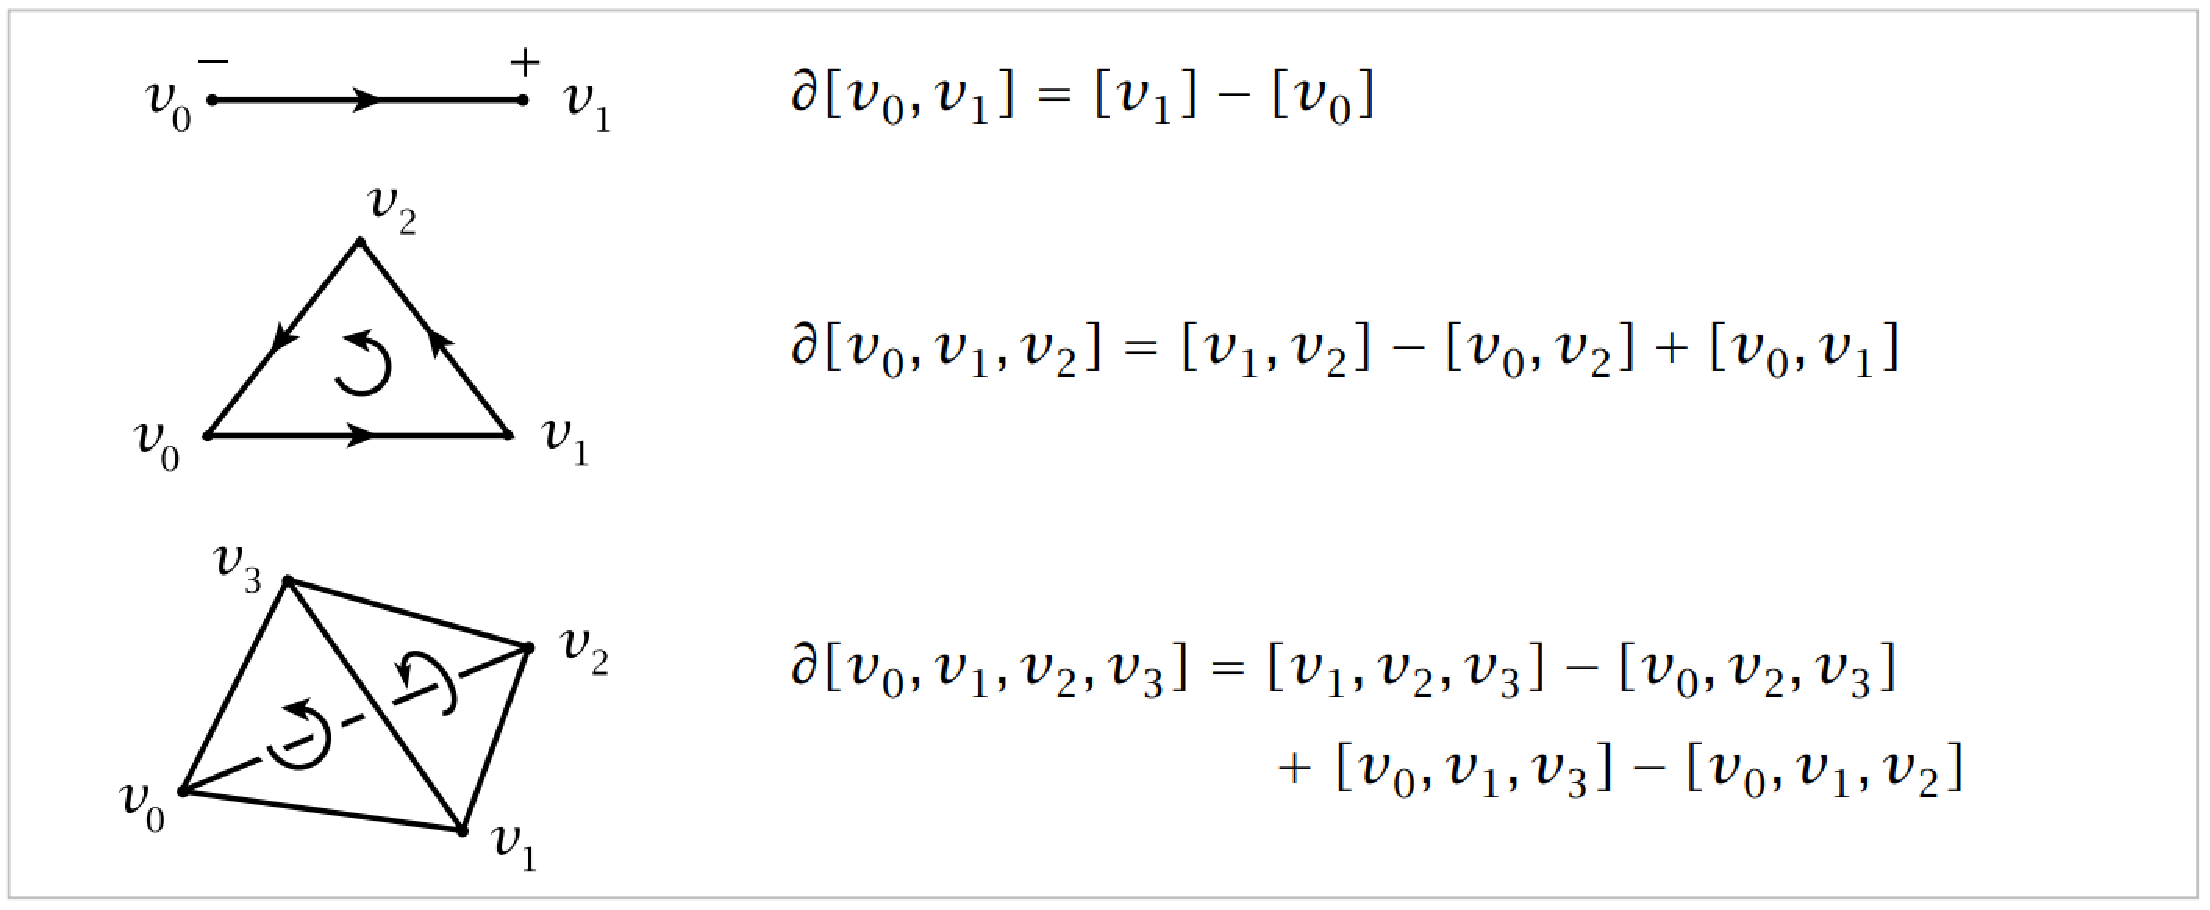
\includegraphics[width=0.9\textwidth]{figures/chap1_2}
\caption[Đồng cấu bờ ]{Đồng cấu bờ 
\label{fig:chap1_2}}
\end{figure}
\indent Với hình học này, chúng ta xác định \emph{đồng cấu bờ} (hay toán tử bờ) \[\partial_n : \Delta_n(X)\rightarrow\Delta_{n-1} (X)\] bằng cách chỉ định các giá trị của nó trên các phần tử cơ sở như sau: \[\partial_n(\sigma_\alpha) = \sum_{i}(-1)^i\sigma_\alpha|[v_0, \cdots,\hat{v}_i,\cdots,v_n]\].

\subsection[Bổ đề]{Bổ đề}
\indent Dãy phức:   \(\Delta_n(X)\xrightarrow[]{\alpha_n}\Delta_{n-1}(X)\xrightarrow[]{\alpha_{n-1}}\Delta_{n-2}(X)\) là bằng không \\
\textbf{Chứng minh}: \\Ta có \[\partial_n(\sigma) = \sum_{i}(-1)^i\sigma|[v_0, \cdots,\hat{v}_i,\cdots,v_n]\] \\
Và từ đây: 
\begin{equation*}\label{eq:pareto mle2}
\begin{aligned}
\partial_{n-1}\partial_n(\sigma) & = \sum_{j<i}(-1)^i(-1)^j\sigma|[v_0, \cdots,\hat{v}_i,\cdots,\hat{v}_j,\cdots,v_n]\\ & + \sum_{j>i}(-1)^i(-1)^{j-1}\sigma|[v_0, \cdots,\hat{v}_i,\cdots,\hat{v}_j,\cdots,v_n] \\
& = 0
\end{aligned}
\end{equation*}
\subsection[Mệnh đề]{Mệnh đề}
\indent Tình huống đại số mà chúng ta có bây giờ là một dãy các đồng cấu của \(abelian\) các nhóm 
\[\cdots\rightarrow C_{n+1} \xrightarrow[]{\partial_{n+1}} C_{n} \xrightarrow[]{\partial_{n}} C_{n-1} \xrightarrow[]{\partial_{n-1}} \cdots \rightarrow C_1 \xrightarrow[]{\partial_{1}} C_0 \xrightarrow[]{\partial_{0}} 0 \]
với \(\partial_n\partial_{n+1} = 0\) , được gọi là một phức dây chuyền. \\
\indent \emph{*Lưu ý: Đã mở rộng thêm 0 ở cuối bên phải với \(\partial_0\)=0} \\
\indent Phương trình \(\partial_n\partial_{n+1} = 0\) tương đương với phép bao hàm Im \(\partial_{n+1} \subset\) Ker \(\partial_n\) , trong đó \(Im\) và Ker là ảnh và hạt nhân. Vì vậy, chúng ta có thể xác định nhóm đồng điều thứ \(n\) phức hợp dây chuyền là nhóm thương \(H_n =\) Ker \(\partial_n / \) Im \(\partial_{n+1}\). Các phần tử của Ker \(\partial_n\) được gọi là chu trình và các phần tử của Im \(\partial_{n+1}\) được gọi là biên. Các phần tử của \(H_n\) của Im \(\partial_{n+1}\) , được gọi là các lớp đồng điều. \\
\indent Trở lại trường hợp \(C_n = \Delta_n(X)\), nhóm đồng điều Ker \(\partial_n/\) Im \(\partial_{n+1}\) sẽ được ký hiệu là \(H_n\Delta(X)\) và được gọi là nhóm đồng điều kỳ dị thứ \(n\) của \(X\) . 
